\documentclass[a4paper]{article}

\usepackage{a4wide}
\usepackage[svgnames]{xcolor}
\usepackage[utf8]{inputenc}
\usepackage{amsmath}
\usepackage{amssymb}
\usepackage{amsthm}
\usepackage{tikz-cd}
\usetikzlibrary{decorations.pathmorphing}
\usepackage{graphicx}
\usepackage{subfig}
\usepackage{hyperref}


\DeclareMathOperator{\id}{id}
\DeclareMathOperator{\inv}{inv}
\DeclareMathOperator{\cano}{cano}
\DeclareMathOperator{\p}{\mathcal{P}}
\DeclareMathOperator{\m}{\mathcal{M}}
\DeclareMathOperator{\op}{\mathcal{O}}



\theoremstyle{definition}
\newtheorem{definition}{Definition}
\newtheorem{proposition}[definition]{Proposition}
\newtheorem{example}[definition]{Example}
\newtheorem{lemma}[definition]{Lemma}
\newtheorem{theorem}[definition]{Theorem}
\newtheorem{corollary}[definition]{Corollary}
\newtheorem{remark}[definition]{Remark}


\begin{document}

\section{Definitions and reminders}

\subsection{Species and Operads}

In all the following $\Bbbk$ is a field, $\mathbb{S}$et is the category of finite sets and bijections, $\underline{\text{$\mathbb{S}$et}}$ the category of finite set and maps and $\mathbb{V}\text{ect}_{\Bbbk}$ the category of $\Bbbk$-vector spaces and linear maps.


\begin{definition}
A \textit{vector} (resp \textit{set}) \textit{species} is a functor from $\mathbb{S}$et to $\mathbb{V}\text{ect}_{\Bbbk}$ (resp $\underline{\text{$\mathbb{S}$et}}$).
More informally, a vector (resp set) species $S$ consists of the following data.
\begin{itemize}
\item For each finite set $V$, a vector space (resp set) $S[V]$.
\item For each bijection of finite sets $\sigma: V\rightarrow V'$, a linear map (resp map) $S[\sigma]:S[V]\rightarrow S[V']$. These maps should be such that $S[\sigma\circ\tau] = S[\sigma]\circ S[\tau]$ and $S[\id] = \id$.
\end{itemize}

% A \textit{sub-species} of a vector species $P$ is a vector species $Q$ such that for each finite set $V$, $Q[V]$ is a sub-space of $P[V]$ and for each bijection of finite sets $\sigma: V\rightarrow V'$, $Q[\sigma] = P[\sigma]|_{Q[V]}$.

A \textit{morphism} between vector (resp set) species is a natural transformation.
More informally, a \textit{morphism} $f: R\rightarrow S$ between vector (resp set) species is a collection of linear maps (resp maps) $f_V : R[V] \rightarrow S[V]$ satisfying the naturality axiom: for each bijection $\sigma: V\rightarrow V'$, $f_{V'}\circ R[\sigma] = S[\sigma]\circ f_V$.

We note $\mathcal{L}$ the functor from set species to vector species defined by $L(S)[V] = \Bbbk S[V]$, where $\Bbbk S[V]$ is the free $\Bbbk$ vector space on $S[V]$, and $L(f)_V$ the linear extension of $f$. We will also note $\Bbbk S$ for $\mathcal{L}(S)$.
\end{definition}

We will use the term species to refer to vector species. For $S$ a species, $V$ a set and $f$ a morphism from $S$ we will note $f$ instead of $f_V$ when no confusion is possible.

We note $1$ the set species defined by $1[V] = \{\emptyset\}$ if $V=\emptyset$ and $1[V] = \emptyset$ else; as well as $X$ the set species defined by $X[V] = \{v\}$ if $V=\{v\}$ and $X[V] = \emptyset$ else.

A partition of $V$ is a subset of $\{\pi_1,\dots, \pi_n\} \subseteq \mathcal{P}(V)\setminus\{\emptyset\}$ such that $\pi_i\cap \pi_j = \emptyset$ for all $i\not = j$ and $\sqcup_i \pi_i = V$. We note $\Pi$ the set species of partitions.

\begin{definition}
Let $R$, $S$, $R'$ and $S'$ be four species and $f:R\rightarrow R'$ and $g:S\rightarrow S'$ two morphisms.
\begin{itemize}
\item The \textit{sum} of $R$ and $S$ is the species $R+ S$ defined by $(R+S)[V] = R[V]\oplus S[V]$ for all finite set $V$ and $(R+S)[\sigma]|_{R[V]} = R[\sigma]$ and $(R+ S)[\sigma]|_{S[V]} = S[\sigma]$ for all finite sets $V,V'$ and bijections $\sigma: V\rightarrow V'$.

The \textit{sum} of $f$ and $g$ is the morphism $f+ g: R +S\rightarrow R'+ S'$ defined by $(f+g)_V = f_V\oplus g_V$.
\item The \textit{product} of $R$ and $S$ is the species $R\cdot S$ defined by $R\cdot S[V] = \bigoplus_{V_1\sqcup V_2 = V} R[V_1]\otimes S[V_2]$ and $R\cdot S[\sigma] = \bigoplus_{V_1\sqcup V_2 = V} R[\sigma|_{V_1}]\otimes S[\sigma|_{V_2}]$.

The \textit{product} of $f$ and $g$ is the morphism $f\cdot g: R\otimes S\rightarrow R'\otimes S'$ defined by $(f\cdot g)_V = \bigoplus_{V_1\sqcup V_2 = V}f_{V_1}\otimes g_{V_2}$.
\item The \textit{Hadamard product} of $R$ and $S$ is the species $R\times S$ defined by $(R\times S)[V] = R[V]\otimes S[V]$ (resp $R[V]\times S[V]$) and $(R\times S)[\sigma] = R[\sigma]\otimes S[\sigma]$ (resp $R[\sigma]\times S[\sigma]$).

The Hadamard product of $f$ and $g$ is the morphism $f\times g$ defined by $(f\times g)_V = f_V\otimes g_V$ (resp $(f\times g)_V = f_V\times g_V$).
\item The \textit{derivative} of $R$ is the species $DR=R'$ defined by $R'[V] = R[V+\{\ast\}]$ where the $\ast$ is a "ghost element" not already in $V$ and $R'[\sigma]= R[\sigma']$ where $\sigma' = \sigma$ on $V$ and $\sigma(\ast) = \ast$. The \textit{$n$-th derivative} of $R$ is the species $D^nR=R^{(n)}$ recursively defined by $D^nR = D(D^{n-1}R)$.
% The \textit{$n$-th derivative} of $R$ is the species $D^nR=R^{(n)}$ defined by $D^nR = R[V+\{\ast_1+\dots+\ast_n\}]$ where the $\ast_i$ are "ghost element" not already in $V$ and $D^nR[\sigma]= R[\sigma']$ where $\sigma' = \sigma$ on $V$ and $\sigma' = \id$ on $\{\ast_1,\dots,\ast_n\}$. The \textit{derivative} of $R$ is the 1-st derivative of $R$ and in this case we will note $\ast=\ast_1$.

The \textit{$n$-derivative} of $f$ is the morphism defined by $(D^nf)_V = f_{V+\{\ast_1,\dots,\ast_n\}}$
\item The \textit{substitution} by $S$ in $R$ is the species $R(S)$ defined by $R(S)[V] = \bigoplus_{P\in\Pi[V]}R[\pi]\bigotimes_{P\in\pi}S(P)$ and $R(S)[\sigma]$ is defined by following the definition of sum and product of species.

The \textit{substitution} by $g$ in $f$ is defined by following the definitions of sum and product of morphisms.
\end{itemize}
We have the same definition on set species by replacing direct sum of vector spaces by disjoint unions of sets and tensor product by Cartesian product.
\end{definition}

Note that we stated these were species and morphisms without checking that these definition were functional and natural. Those verifications can be found in (ref...). These definitions are compatible with $\mathcal{L}$ i.e $\mathcal{L}(R+S) = \mathcal{L}(R)+\mathcal{L}(S)$, $\mathcal{L}(f+g) = \mathcal{L}(f)+\mathcal{L}(g)$, $\mathcal{L}(R\cdot S) = \mathcal{L}(R)\cdot \mathcal{L}(S)$ etc.


% In the following, in order to avoid confusions when referring to ghost element, we will consider a slightly different product of species: $D^nR\otimes D^mS[V] = \bigoplus_{V_1\sqcup V_2 = V} D^nR[V_1]\otimes S[\sigma_{V_2}]D^mS[V_2]$ where $\sigma_{V_2}$ is the identity on $V_2$ and sends $\ast_i$ on $\ast_{i+m}$ for $i\in [n]$.

When no confusion is possible we will note $S$ instead of $\id_S$.

\begin{definition}
A \textit{linear operad} is a triplet $(\op,\eta,e)$ where:
\begin{itemize}
\item $\mathcal{O}$ is a vector species,
\item $\eta$ is a morphism of vector species $\mathcal{O}(\mathcal{O})\rightarrow \mathcal{O}$,
\item $e$ is a morphism of vector species $X \rightarrow \op$.
\end{itemize}
The two morphisms $\eta$ and $e$ should furthermore satisfy the associativity and naturality axioms, i.e the two following diagrams commute, where $\alpha$, $\rho$ and $\lambda$ are the structural morphisms of the monoidal category of vector species (ref...) .
\begin{center}
\begin{tikzcd}
\op(\op(\op)) \arrow[r, "\op(\eta)"] \arrow[d, "\alpha"]& \op(\op) \arrow[r, "\eta"] & \op \\
(\op(\op))(\op) \arrow[r, "\eta(\op)"] & \op(\op) \arrow[ur, "\eta"]
\end{tikzcd}
\end{center}
\begin{center}
\begin{tikzcd}
\op(X) \arrow[r, "\op(e)"] \arrow[rd, "\rho"] & \op(\op) \arrow[d, "\eta"] & X(\op) \arrow[l, "e(\op)" swap]\arrow[dl, "\lambda" swap]\\
& \op 
\end{tikzcd}
\end{center}
\end{definition}

We will use the term operad to refer to linear operad.

Let $S$ be a species. We call \textit{partial product} on $S$ a morphism $\circ_{\ast} :S'\cdot S \rightarrow S$. A partial product naturally generalise to families of $n$ morphisms $D^nS\otimes D^mS \rightarrow D^{n+m-1}S$ by the injections
\begin{align*}
D^nS[V_1]\otimes D^mS[V_2] &\cong S'[V_1+\{\ast_1,\dots,\ast_{i-1},\ast_{i+1},\dots,\ast_n\}]\otimes S[V_2+\{\ast_1',\dots\ast_m'\}] \\
&\hookrightarrow (S'\cdot S)[V_1+V_2+\{\ast_1,\dots, \ast_{i-1},\ast_{i+1},\dots,\ast_n\} + \{\ast_1',\dots\ast_m'\}].
\end{align*} 

\begin{proposition}
\label{pp}
Let $\op$ be a species equipped with a \textit{partial product} $\circ_{\ast}:\op'\cdot\op\rightarrow \op$ and a morphism $e:X \rightarrow \op$ such that the following diagrams commute.
\begin{center}
\begin{tikzcd}
\op''\cdot\op^2 \arrow[r, "\circ_{\ast_1}"] \arrow[d, "\circ_{\ast_2}\circ\id\cdot\tau"] & \op'\cdot\op \arrow[d, "\circ_{\ast_2}"] & &
\op'\cdot \op'\cdot\op \arrow[r, "\circ_{\ast_1}\cdot\id"] \arrow[d, "\id\cdot\circ_{\ast_2}"] & \op'\cdot\op \arrow[d, "\circ_{\ast_2}"] \\
\op'\cdot \op \arrow[r, "\circ_{\ast_1}"] & \op & & 
\op'\cdot \op \arrow[r, "\circ_{\ast_1}"] & \op
\end{tikzcd}
\end{center}
\begin{center}
\begin{tikzcd}
\op'\cdot X \arrow[r, "\op'\cdot e"] \arrow[rd, "p"] & \op'\cdot\op \arrow[d, "\circ_{\ast}"] & X'\cdot \op \arrow[l, "e'\cdot \op" swap]\arrow[dl, "\cong" swap]\\
& \op 
\end{tikzcd}
\end{center}
where $\tau_V:x\otimes y\in \op^2[V] \mapsto y\otimes x\in \op^2[V]$ and $p_V: x\otimes \emptyset_{\{v\}} \mapsto \op[\ast\mapsto v](x)$ with $\ast\mapsto v: V\setminus\{v\} + \{\ast\}\rightarrow V$ the bijection that sends $\ast$ on $v$ and is the identity on $V\setminus\{v\}$.
Then $\op$ has an operad structure $(\op,\eta,e)$ uniquely determined by $\circ_{\ast}$.
\end{proposition}


\subsection{Multisets, graphs and co}

Let $V$ be a set. A \textit{multiset} $m$ over $V$ is a set of couples $\{(v,m(v))\,|\, v\in V\}$ in $V\times\mathbb{N}^*$. We call $V$ the domain of $m$ and note $D(m)=V$. We say that $v$ is in $m$ and note $v\in m$ if $v\in D(m)$. For any element $v$ not in the domain of $m$, we note $m(v) = 0$.

We note $\m(V)$ the set of multisets with domain in $\p(V)$, $\m_k(V)$ the set of elements of $\m(V)$ of cardinality $k$ (the cardinality of a multiset $m$ over $V$ being $\sum_{v\in V} m(v)$) and $\m(V)^*$ the set of multisets with domain in $\p(V)^* = \p(V)\setminus\{\emptyset\}$. We indentify sets with multisets constant equal to 1.

%In addition to the usual way to represent maps, we also use two different notations for subsets: the set notation and the couple notation. For example the multiset $m$ over $\{a,b,c\}$ defined by $m(a) = 2$, $m(b) = 1$ and $m(c)=2$ will also be noted as $\{a,a,b,c,c\}$ or $\{(a,2),(b,1),(c,2)\}$. We will say that $v$ is an element of $m$ and $v \in m$ if $v\in D(m)$, with $D(m)$ the domain of $m$.

%Note $\p_k(V_1)$ the set of subsets of cardinality $k$ of $V_1$ and $\m_k(V_1)$ the set of multisets of cardinality $k$ (the cardinality of a multiset $m$ over $V_1$ being $\sum_{v\in V_1} m(v)$) as well as $\p(V_1)^* = \p(V_1)\setminus\{\emptyset\}$ and $\m(V_1)^* = \m(V_1)\setminus\{\emptyset\}$.
%We note $Dec_k(m)$ the set of decomposition of lenght 2 of $m$.

% Let $m_1$ and $m_2$ be two multisets and $V$ a set.
% \begin{itemize}
% \item We note $m_1\oplus m_2$ the multiset over $D(m_1)\cup D(m_2)$ defined by $m_1\oplus m_2(v) = m_1(v) + m_2(v)$ (where we define $m_i(v) = 0$ if it is not already defined).
% \item We note $m_1\cap V$ the multiset over $D(m)\cap V$ defined by $m_1\cap V(v)= m_1(v)$ for $v\in D(m)\cap V$.
% \end{itemize}
For $m$ a multiset and $V$ a set, we note $m\cap V = m\cap V\times\mathbb{N}^*$. If $m'$ is an other multiset, we call the union of $m$ and $m'$ the multiset $\{(v,m(v)+m'(v))\,|\, v\in D(m)\cup D(m')\}$ where $m(v) = 0$ if $v\not in D(m)$ and $m'(v) = 0$ if $v\not \in D(m')$.
A \textit{decomposition} of a mutliset $m$ is a tuple of multisets $(m_1,\dots, m_k)$ such that $\bigcup D(m_i) = D(m)$ and $m(v) = m_i(v)$ for all $v\in D(m)$.

\begin{definition}
Let $V$ de a set. A \textit{multi-hypergraph} over $V$ is a multiset with domain in $\m(V)^*$. In this context the elements of $V$ are called \textit{vertices}, the elements of a multi-hypergraphs are called \textit{edges} and the elements of an edge are called its \textit{ends}. A vertex contained in the domain of no edge is called \textit{isolated vertex}. We note $MHG$ the set species of multi-hypergraphs.

A \textit{hypergraph} is a multi-hypergraph whose edges are sets. A \textit{mutltigraph} is a multi-hypergraph whose edges have cardinality 2. A \textit{graph} is a multi-hypergraph which is a hypergraph and a multigraph at the same time. Note $MHG$, $HG$, $MG$ and $G$ the set species corresponding to these structures.

 An \textit{orientation} of a multi-hypergraph $h$ is given by a decomposition of size 2 $(e_s,e_t)$ for each edge $e\in h$. The elements of $e_s$ and $e_t$ are respectively called \textit{source ends} and \textit{target ends} of $e$. An \textit{oriented multi-hypergraph} (resp \textit{oriented hypergraph}, \textit{oriented multigraph}, \textit{oriented graph}) is a multi-hypergraph (resp hypergraph, multigraph, graph) with an orientation. An oriented multi-hypergraph over $V$ can also be seen as a multiset with domain in $(\m(V)^*)^2$. The elements of an oriented multi-hypergraph are then called oriented edges.
\end{definition}

In contrast with the standard definition, here the sole difference between graphs and multigraphs is that multigraphs can have loops while graphs no; but in both case we accept repetition of edges. The notion of orientation for a graph also differs from the usual one where each edge has exactly one source and one target.
\begin{figure}[htbp]
\begin{center}
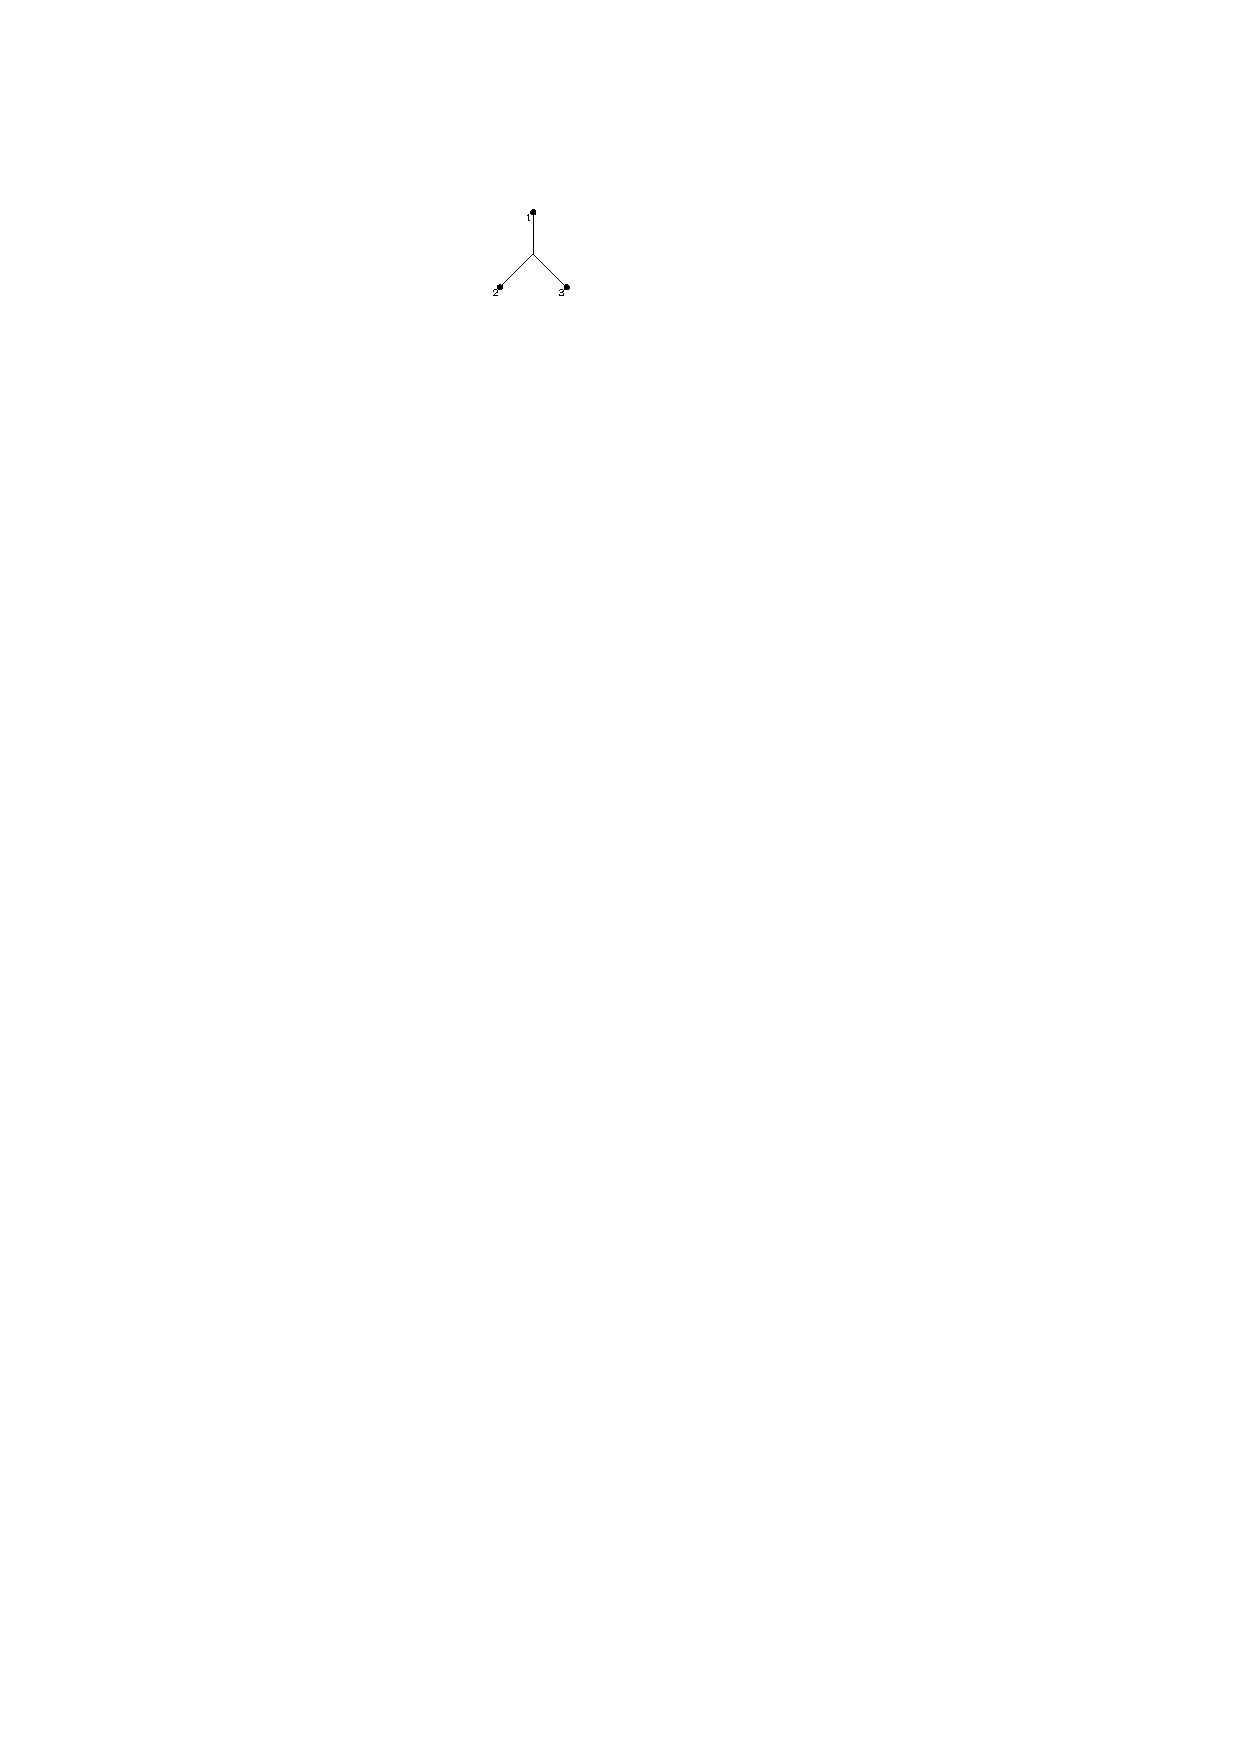
\includegraphics[scale=1.5]{fig/he1}
\hspace{2cm}
{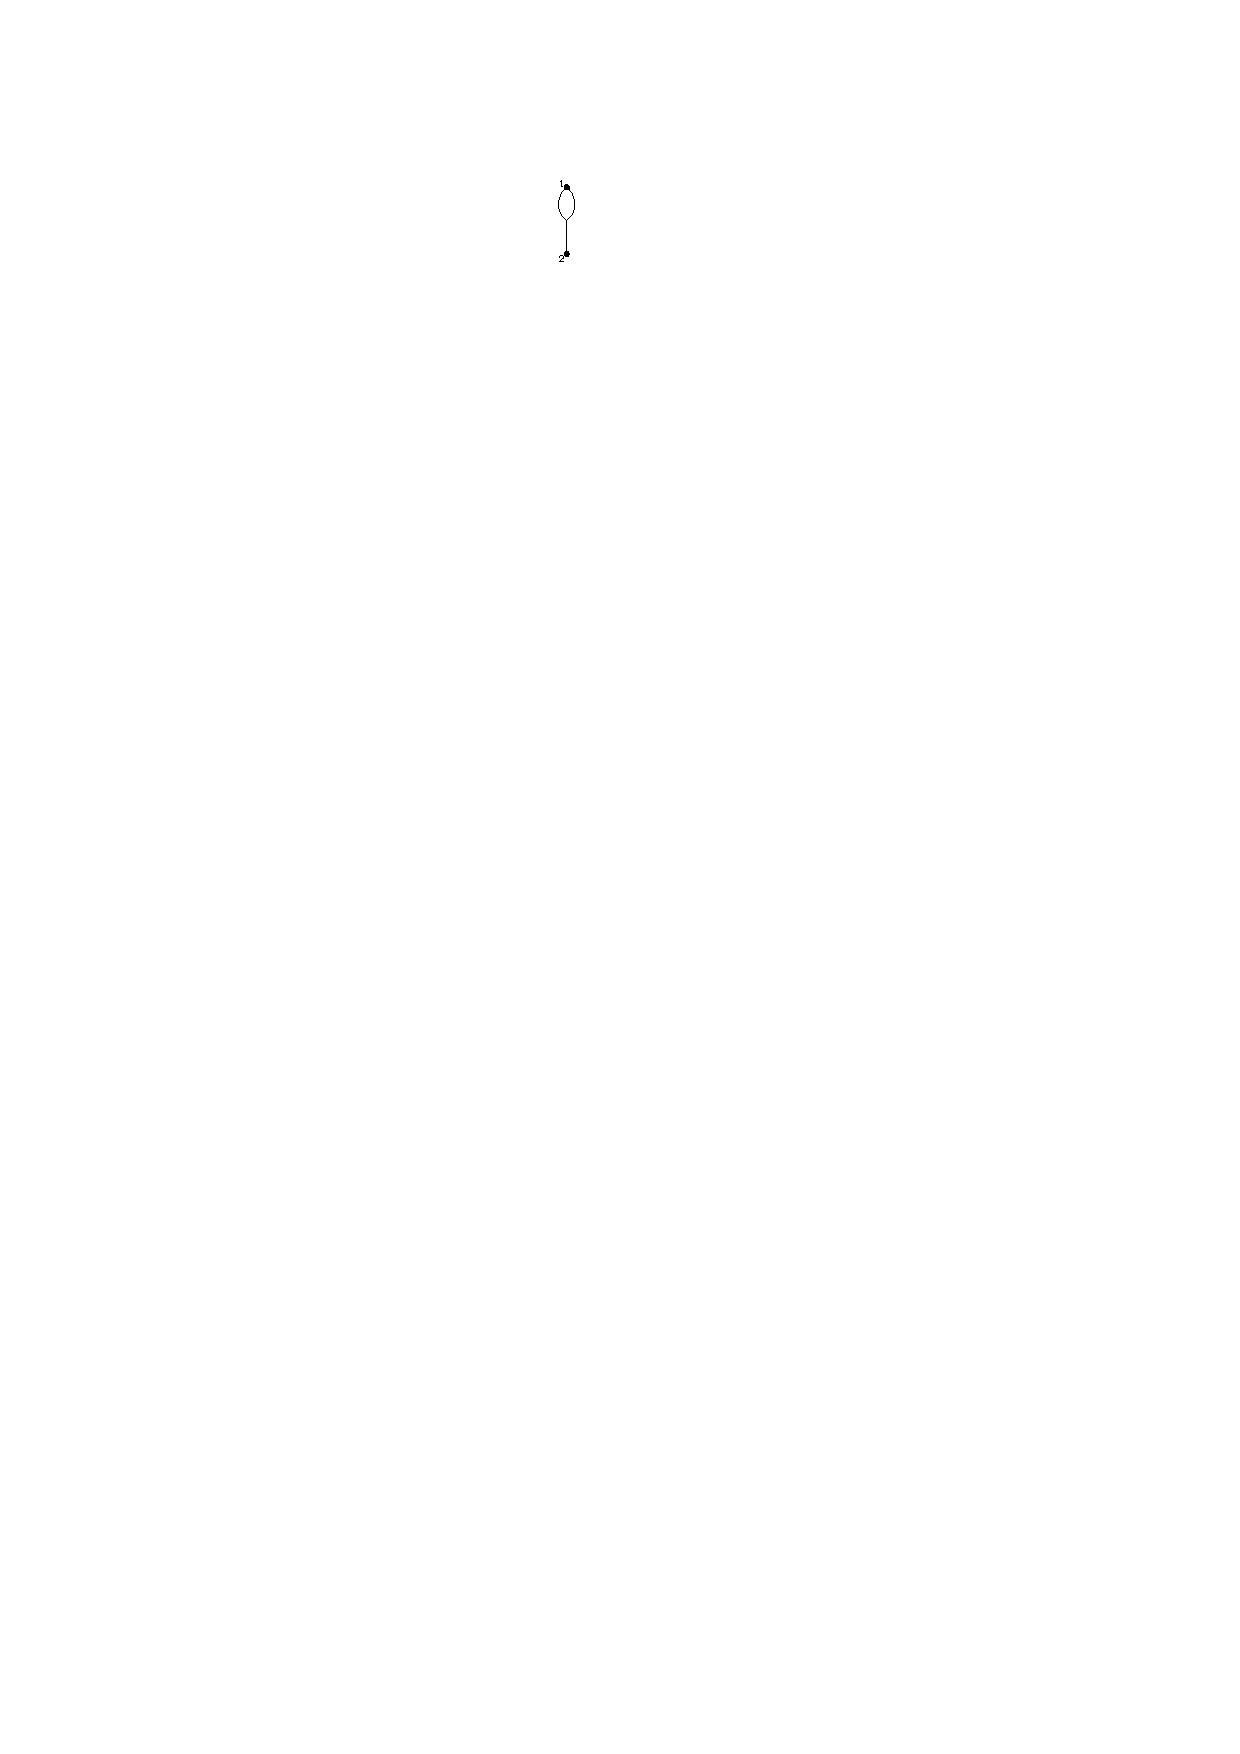
\includegraphics[scale=1.5]{fig/he2}}
\hspace{2cm}

\includegraphics[scale=1.5]{fig/he3}
\caption{Three edges of cardinality 3.}
\label{e3}

\end{center}
\end{figure}
\begin{figure}[htbp]
\begin{center}
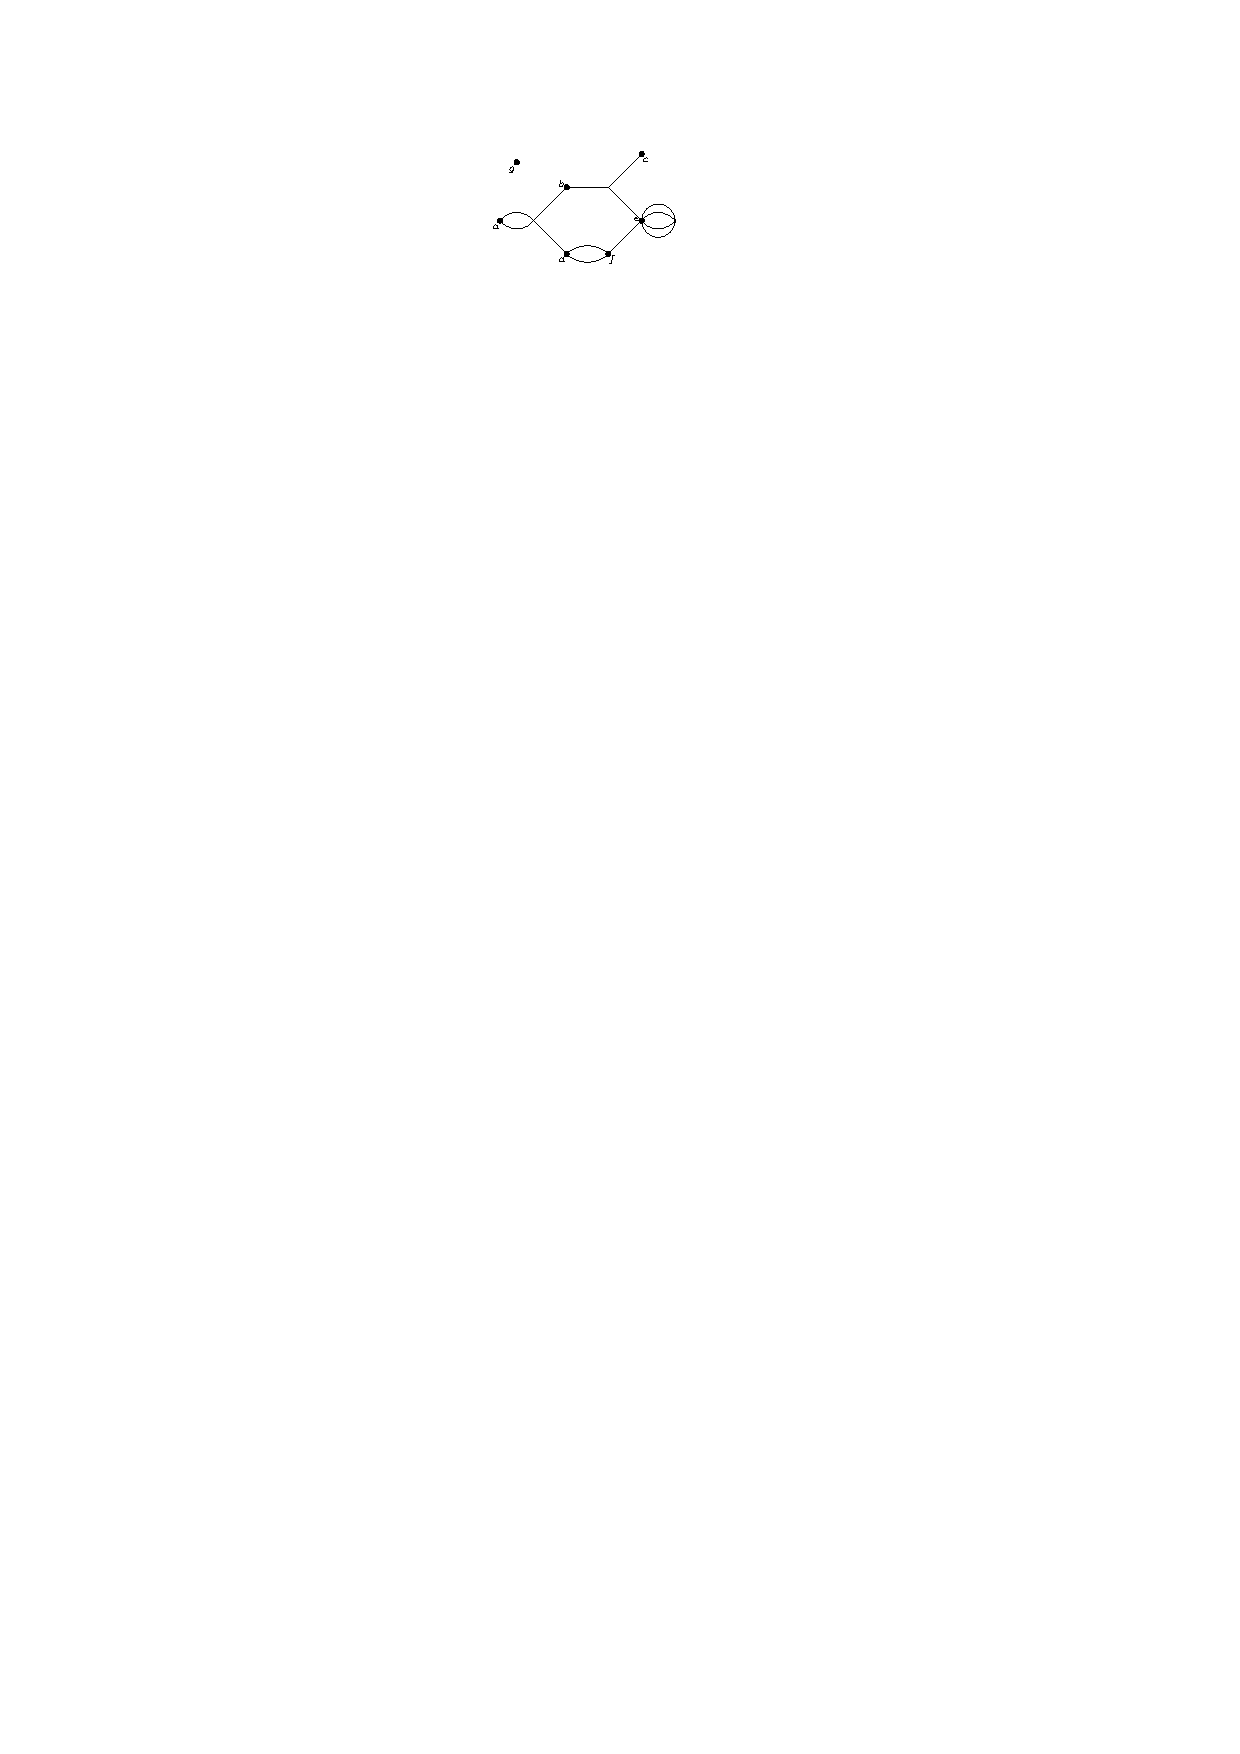
\includegraphics[scale=1.5]{fig/mhg1}
\caption{A mulit-hypergrah over $\{a,b,c,d,e,f,g\}$.}
\label{mhg}
\end{center}
\end{figure}


\begin{example}
We represented the three edges $\{(1,1),(2,1),(3,1)\}$, $\{(1,2),(2,1)\}$ and $\{(1,3)\}$ in Figure \ref{e3} and the multi-hypergraph $$\{(\{(a,2),(b,1),(d,1)\},1),(\{(b,1),(c,1),(e,1)\},1),(\{e,4\},1),(\{(e,1),(f,1)\},1),(\{(d,1),(e,1)\},2)\}$$ over $\{a,b,c,d,e,f,g\}$ in Figure \ref{mhg}.
\end{example}

Let $S$ one of the set species $HMG$, $HG$, $MG$ or $G$. We note $S_c$ the set subspecies of $S$ of connected elements, $S_{or}$ the set species of oriented elements and $S_{orc}$ the set subspecies of $S_{or}$ of connected elements. We note $F$ the set species of forest, $T=F_c$ the set species of trees, $F_{or}$ the set species of oriented forest, $T_{or}$ the set species of oriented trees and $A$ the set species of rooted trees.

% Given a set species $S$ the \textit{pointing of $S$} is the set species $S^{\bullet}$ given by $S^{\bullet}[V] = S[V]\times V$. Given $(h,r)\in MHG_c^{\bullet}$, we have a canonical orientation of $h$ defined iteravely as follow.
% \begin{itemize}
% \item For each edge $e$ containing $r$ the domain $D(e_t)$ of $e_t$ is $\{r\}$ and $e_t(r) = e(r)$.
% \item For each edge $e$ not already oriented containing vertices which are in an oriented edge, let $V$ be this set of vertices. Then $D(e_t) = V$ and $e_t(v) = e(v)$.
% \end{itemize}
% Remark that if $h$ is a tree, this gives us the rooted tree with root $r$ and underlying tree $h$. We note $O_r(h)$ the oriented multi-hypergraph thus obtained and $O$ the morphism $HMG_c^{\bullet} \rightarrow HMG_{orc}^{\bullet}: (h,r) \mapsto (O_r(h),r)$.

% $\Bbbk G[V]$ is naturally equipped with a scalar product $\langle,\rangle_V$ defined by $\langle g_1, g_2\rangle_V = \delta_{g_1,g_2}$ for $g_1,g_2\in G[V]$. In the following we will omit the $V$ index and note $\langle,\rangle$


\section{Augmented multi-hypergraphs}

\begin{definition}
Let $A$ be a set and $V$ a finite set. An \textit{$A$-augmented edge over $V$} is an element of $\m(V\times A)$ and an \textit{$A$-augmented multi-hypergraph over $V$} is a multiset of $A$-augmented edges. Note $A\text{-}MHG$ the set species of $A$-augmented multi-hypergraphs.
\end{definition}

\begin{example}
...
\end{example}

Let $A$ be a set and $V$ a finite set. For $a\in A$ and $V\in v$, we will note:
\begin{itemize}
\item $v_a = (a,v)$ for $v\in V$ and $a\in A$,
\item $\prod_{(v,a)\in e} v_a^{e((v,a))}$ for an $A$-augmented edge $e$ over $V$,
\item $\emptyset_V$ the empty $A$-augmented multi-hypergraph over $V$,
\item $\bigoplus_{e_i\in h}e_i^{\oplus h(e_i)}$ for an $A$-augmented multi-hypergraph $h$.
\end{itemize}
With these notations we can see $A$-augmented edges over $V$ as monomials on the set of variables $\{v_a\,|\, v\in V,  a\in A\}$ and non empty $A$-augmented multi-hypergraphs over $V$ as polynomials with positive integer coefficients on the same set of variables. The binary operation $\oplus$ over $A$-augmented multi-hypergraphs can then be interpreted as the union of multisets of edges or the sum over polynomials. Note that we used $\oplus$ for the sum of polynomials / union of multisets such as to not confuse it with the $+$ of $\Bbbk A\text{-}MHG[V]$. In this context, the sum of polynomials $\oplus$ and the product of polynomials $\cdot$ are distributive over the sum of vectors $+$.

\begin{example}
...
\end{example}

Note $V = \{v_1,\dots, v_n\}$ and $A=\{a_1, a_2, \dots\}$. Let be $h\in A\text{-}MHG[V]$, $1\leq i_1 <\dots < i_k\leq n$ be $k\leq n$ integers, $V'$ be a finite set disjoint of $V$ and for every $1\leq j\leq k$, $a\in A$, $\emptyset\subsetneq V_{j,a} \subseteq V'$. We note $h|_{\{ {v_{i_j}}_a \leftarrow V_{j,a}\}_{1\leq j\leq k, a\in A}}$ the substitution of every $v_{i_j}\in V$ by $\sum_{v\in V_{j,a}} v_a$ in the polynomial $h$, i.e: $$h(\dots, v_{i_1a_1},\dots, v_{i_ja_1},\dots)|_{\{ v_{i_ja} \leftarrow V_{j,a}\}_{1\leq j\leq k, a\in A}} = h(\dots, \sum_{v\in V_{1,a_1}} v_{a_1}, \dots, \sum_{v\in V_{j,a_1}} v_{a_1}, \dots).$$
In the case of the empty $A$-augmented multi-hypergraphs over $V$ we note $\emptyset_V|_{\{ {v_{i_j}}_a \leftarrow V_{j,a}\}_{1\leq j\leq k, a\in A}} = \emptyset_{V\setminus\{v_{i_j}\}_{1\leq j\leq k}}$.

We note $\mathcal{F}_A$ the set of maps from $A$ to $\mathcal{P}\setminus\{\emptyset\}$.
Let $V_1$ and $V_2$ be two finite disjoint sets. For $(h_1,f_1)\in (A\text{-}MHG\times \mathcal{F}_A)'[V_1]$ and  $(h_2,f_2)\in (A\text{-}MHG\times \mathcal{F}_A)[V_2]$ we define the element of $\Bbbk((A\text{-}MHG\times\mathcal{F}_A)[V_1+V_2]$:
$$ (h_1,f_1)\circ_{\ast}(h_2,f_2) = \left(h_1|_{\{\ast_a\leftarrow f_2(a)\}_{a\in A}}\oplus h_2, f_1\circ_\ast f_2: a\rightarrow\left\{\begin{array}{cl}
f_1(a)  & \text{if $\ast\not\in f_1(a)$},    \\ 
f_1(a)\setminus\{\ast\} + f_2(a)  & \text{else.}\end{array}\right.\right)$$
where $(\sum_i h_i, f) = \sum_i(h_i,f)$.
Let us also define $e:\Bbbk X \rightarrow \Bbbk (A\text{-}MHG\times \mathcal{F}_A)$ by $e_{V}(v) = (\emptyset_{\{v\}},A\mapsto\{v\})$ if $V=\{v\}$ and $e_V = 0$ else.

\begin{lemma}
\label{opfunc}
The partial product $\circ_{\ast}$ on $\mathcal{F}_A$ and the morphism $e:X \rightarrow \Bbbk \mathcal{F}_A$ defined by $e_{V}(v) = A\mapsto\{v\}$ if $V=\{v\}$ and $e_V = $ else are such that the diagrams of Proposition \ref{pp} commute and hence define an operad structure on $\mathcal{F}_A$
\end{lemma}

\begin{proof}
Since $\mathcal{F}_A[\sigma](f) = \sigma\circ f$ it is easy to see that $\circ_{\ast}$ is a morphism of species. Let now be $V_1$, $V_2$ and $V_3$ three disjoint sets.
\begin{itemize}
\item Let be $f_1\in\mathcal{F}_A[V_1+\{\ast_1,\ast_2\}]$, $f_2\in \mathcal{F}_A[V_2]$ and $f_3\in \mathcal{F}_A[V_3]$. Then:
\begin{align*}
(f_1\circ_{\ast_1} f_2)\circ_{\ast_2} f_3 &= a\mapsto\left\{\begin{array}{cl}
f_1(a)  & \text{if $\ast_1\not\in f_1(a)$},    \\ 
f_1(a)\setminus\{\ast_1\} + f_2(a)  & \text{else.}\end{array}\right. \circ_{\ast_2} f_3 \\
&= a\mapsto\left\{\begin{array}{cl}
f_1(a)  & \text{if $\ast_1\not\in f_1(a)$ and $\ast_2\not\in f_2(a)$},    \\
f_1(a)\setminus\{\ast_2\} + f_3(a)  & \text{if $\ast_1\not\in f_1(a)$ and $\ast_2\in f_2(a)$},    \\ 
f_1(a)\setminus\{\ast_1\} + f_2(a)  & \text{if $\ast_1\in f_1(a)$ and $\ast_2\not\in f_2(a)$},    \\ 
f_1(a)\setminus\{\ast_1,\ast_2\} + f_2(a) + f_3(a)  & \text{if $\ast_1\in f_1(a)$ and $\ast_2\in f_2(a)$}.\end{array}\right. \\
&= a\mapsto\left\{\begin{array}{cl}
f_1(a)  & \text{if $\ast_2\not\in f_1(a)$},    \\ 
f_1(a)\setminus\{\ast_1\} + f_3(a)  & \text{else.}\end{array}\right. \circ_{\ast_1} f_2 \\
&= (f_1\circ_{\ast_2} f_3)\circ_{\ast_1} f_2
\end{align*}
\item Let be $f_1\in\mathcal{F}_A[V_1+\{\ast_1\}]$, $f_2\in \mathcal{F}_A[V_2+\{\ast_2\}]$ and $f_3\in \mathcal{F}_A[V_3]$. Then:
\begin{align*}
(f_1\circ_{\ast_1} f_2)\circ_{\ast_2} f_3 &= a\mapsto\left\{\begin{array}{cl}
f_1(a)  & \text{if $\ast_1\not\in f_1(a)$},    \\ 
f_1(a)\setminus\{\ast_1\} + f_2(a)  & \text{else.}\end{array}\right. \circ_{\ast_2} f_3 \\
&= a\mapsto\left\{\begin{array}{cl}
f_1(a)  & \text{if $\ast_1\not\in f_1(a)$ and $\ast_2\not\in f_2(a)$},    \\
f_1(a)  & \text{if $\ast_1\not\in f_1(a)$ and $\ast_2\in f_2(a)$},    \\ 
f_1(a)\setminus\{\ast_1\} + f_2(a)  & \text{if $\ast_1\in f_1(a)$ and $\ast_2\not\in f_2(a)$},    \\ 
f_1(a)\setminus\{\ast_1\} + f_2(a)\setminus\{\ast_2\} + f_3(a)  & \text{if $\ast_1\in f_1(a)$ and $\ast_2\in f_2(a)$}.\end{array}\right. \\
&= f_1\circ_{\ast_1} \left\{\begin{array}{cl}
f_2(a)  & \text{if $\ast_2\not\in f_2(a)$},    \\ 
f_2(a)\setminus\{\ast_2\} + f_3(a)  & \text{else.}\end{array}\right. \\
&= f_1\circ_{\ast_1}(f_2\circ_{\ast_2} f_3)
\end{align*}
\item Let be $f\in \mathcal{F}_1[V_1]$ and $f'\in\mathcal{F}_A[V_1+\{\ast\}]$. Then $A\mapsto\{\ast\}\circ_{\ast} f= f$ and $f'\circ_{\ast} A\mapsto \{v\}= (\ast\mapsto v )\circ f'$.
\end{itemize}
\end{proof}

\begin{lemma}
\label{oppol}
Let $A=\{a_1,\dots\}$ be a set, $V$, $V_1$ and $V_2$ pairwise disjoint finte sets.
\begin{itemize}
\item If $h\in A\text{-}MHG[V_1+\{\ast_1,\ast_2\}]$ and $f_1\in \mathcal{F}_A[V_1]$ and $f_2\in \mathcal{F}_A[V_2]$ then $h|_{\{\ast_{1a}\leftarrow f_1(a)\}_{a\in A}}|_{\{\ast_{2a}\leftarrow f_2(a)\}_{a\in A}} = h|_{\{\ast_{2a}\leftarrow f_2(a)\}_{a\in A}}|_{\{\ast_{1a}\leftarrow f_1(a)\}_{a\in A}}$.
\item If $h\in A\text{-}MHG[V_1+\{\ast_1\}]$ and $f_1\in \mathcal{F}_A[V_1+\{\ast_2\}]$ and $f_2\in \mathcal{F}_A[V_2]$ then $h|_{\{\ast_{1a}\leftarrow f_1(a)\}_{a\in A}}|_{\{\ast_{2a}\leftarrow f_2(a)\}_{a\in A}} = h|_{\{\ast_{1a}\leftarrow f_1\circ_{\ast_2} f_2(a)\}_{a\in A}}$
\end{itemize}
\end{lemma}

\begin{proof}
This is just saying that the composition of multivariate polynomials is "symmetric" and associative.
\begin{itemize}
\item \begin{align*}
h_1(\dots, \ast_{1a_1},\dots,\ast_{2a_1},\dots)&|_{\{\ast_{1a}\leftarrow f_1(a)\}_{a\in A}}|_{\{\ast_{2a}\leftarrow f_2(a)\}_{a\in A}} \\
&= h_1(\dots, \sum_{v\in f_1(a_1)}v_{a_1},\dots, \ast_{2a_1},\dots)|_{\{\ast_{2a}\leftarrow f_2(a)\}_{a\in A}} \\
&= h_1(\dots, \sum_{v\in f_1(a_1)}v_{a_1},\dots, \sum_{v\in f_2(a_1)}v_{a_1},\dots) \\
&= h_1(\dots, \ast_{1a_1},\dots, \sum_{v\in f_2(a_1)}v_{a_1},\dots)|_{\{\ast_{1a}\leftarrow f_1(a)\}_{a\in A}} \\
&= h_1(\dots, \ast_{1a_1},\dots,\ast_{2a_1},\dots)|_{\{\ast_{2a}\leftarrow f_2(a)\}_{a\in A}}|_{\{\ast_{1a}\leftarrow f_1(a)\}_{a\in A}}
\end{align*}
\item \begin{align*}
h_1(\dots,\ast_{1a_1},\dots)&|_{\{\ast_{1a}\leftarrow f_1(a)\}_{a\in A}}|_{\{\ast_{2a}\leftarrow f_2(a)\}_{a\in A}} \\
&= h_1(\dots, \sum_{v\in f_1(a_1)}v_{a_1},\dots)|_{\{\ast_{2a}\leftarrow f_2(a)\}_{a\in A}} \\
&= h_1(\dots, \sum_{v\in f_1(a_1)\setminus\{\ast_2\}}v_{a_1} + \delta_{\ast_2\in f_1(a_1)}\sum_{v\in f_2(a_1)}v_{a_1},\dots) \\
&= h_1(\dots, \sum_{v\in f_1\circ_{\ast_2}f_2(a_1)}v_{a_1},\dots) \\
&= h_1(\dots,\ast_{1a_1},\dots)|_{\{\ast_{1a}\leftarrow f_1\circ_{\ast_2}f_2(a)\}_{a\in A}}
\end{align*}
where $\delta_{\ast_2\in f_1(a_1)} =1$ if $\ast_2\in f_1(a_1)$ and $\delta_{\ast_2\in f_1(a_1)} =0$ else.
\end{itemize}
\end{proof}

\begin{theorem}
The partial product $\circ_{\ast}$ and the morphism $e$ are such that the diagrams of Proposition \ref{pp} commute and hence define an operad structure on $\Bbbk A\text{-}MHG\times\mathcal{F}_A$ as well as all its subspecies stable under partial product. 
\end{theorem}

\begin{proof}
We must first show that $\circ_{\ast}$ is a morphism of species. Let $V_1$ and $V_2$ be two finite disjoint sets, $(h_1,f_1)\in (A\text{-}MHG\times \mathcal{F}_A)'[V_1]$ and $(h_2,f_2)\in (A\text{-}MHG\times \mathcal{F}_A)[V_2]$ and $\sigma: V_1\sqcup V_2\rightarrow V$ a bijection. Then,
\begin{align*}
(A\text{-}MHG\times\mathcal{F}_A)[\sigma]&((h_1,f_1)\circ_{\ast}(h_2,f_2)) \\
&= (A\text{-}MHG\times\mathcal{F}_A)[\sigma]((h_1|_{\{\ast_a\leftarrow f_2(a)\}_{a\in A}}\oplus h_2, f_1\circ_{\ast}f_2) \\
&= (A\text{-}MHG[\sigma](h_1|_{\{\ast_a\leftarrow f_2(a)\}_{a\in A}}\oplus h_2), \mathcal{F}_A[\sigma](f_1\circ_{\ast} f_2)) \\
&= (A\text{-}MHG'[\sigma_{|V_1}](h_1)|_{\{\ast_a\leftarrow \sigma_{|V_2}(f_2(a))\}_{a\in A}}\oplus A\text{-}MHG[\sigma_{|V_2}](h_2), \mathcal{F}_A'[\sigma_{|V_1}](f_1)\circ_{\ast}\mathcal{F}_A[\sigma_{|V_2}](f_2)) \\
&= (A\text{-}MHG\times\mathcal{F}_A)'[\sigma_{}]((h_1,f_1)) \circ_{\ast}(A\text{-}MHG\times\mathcal{F}_A)[\sigma]((h_2,f_2)) 
\end{align*}

Let now be $V_1$, $V_2$ and $V_3$ three disjoint sets and note $A=\{a_1,\dots\}$.
\begin{itemize}
\item Let be $(h_1,f_1)\in (A\text{-}MHG\times \mathcal{F}_A)[V_1+\{\ast_1,\ast_2\}]$,  $(h_2,f_2)\in (A\text{-}MHG\times \mathcal{F}_A)[V_2]$ and $(h_3,f_3)\in(A\text{-}MHG\times \mathcal{F}_A)[V_3]$. Then:
\begin{align*}
((h_1,f_1)&\circ_{\ast_1}(h_2,f_2))\circ_{\ast_2} (h_3,f_3) \\
&= (h_1|_{\{\ast_{1a}\leftarrow f_2(a)\}_{a\in A}}\oplus h_2, f_1\circ_{\ast_1}f_2)\circ_{\ast_2}(h_3,f_3) \\
&= (h_1|_{\{\ast_{1a}\leftarrow f_2(a)\}_{a\in A}}|_{\{\ast_{2a}\leftarrow f_3(a)\}_{a\in A}}\oplus h_2|_{\{\ast_{2a}\leftarrow f_3(a)\}_{a\in A}}\oplus h_3, (f_1\circ_{\ast_1}f_2)\circ_{\ast_2}f_3) \\
&= (h_1|_{\{\ast_{2a}\leftarrow f_3(a)\}_{a\in A}}|_{\{\ast_{1a}\leftarrow f_2(a)\}_{a\in A}}\oplus h_3|_{\{\ast_{1a}\leftarrow f_2(a)\}_{a\in A}}\oplus h_2, (f_1\circ_{\ast_2}f_3)\circ_{\ast_1}f_2) \\
&= (h_1|_{\{\ast_{2a}\leftarrow f_3(a)\}_{a\in A}}\oplus h_3, f_1\circ_{\ast_2}f_3)\circ_{\ast_1}(h_2,f_2) \\
&= ((h_1,f_1)\circ_{\ast_2}(h_3,f_3))\circ_{\ast_1} (h_2,f_2),
\end{align*}
where the third equality comes from Lemma \ref{opfunc} and Lemma \ref{oppol}.
\item Let be $(h_1,f_1)\in (A\text{-}MHG\times \mathcal{F}_A)[V_1+\{\ast_1\}]$,  $(h_2,f_2)\in (A\text{-}MHG\times \mathcal{F}_A)[V_2+\{\ast_2\}]$ and $(h_3,f_3)\in(A\text{-}MHG\times \mathcal{F}_A)[V_3]$. Then:
\begin{align*}
((h_1,f_1)&\circ_{\ast_1}(h_2,f_2))\circ_{\ast_2} (h_3,f_3) \\
&= (h_1|_{\{\ast_{1a}\leftarrow f_2(a)\}_{a\in A}}\oplus h_2, f_1\circ_{\ast_1}f_2)\circ_{\ast_2}(h_3,f_3) \\
&= (h_1|_{\{\ast_{1a}\leftarrow f_2(a)\}_{a\in A}}|_{\{\ast_{2a}\leftarrow f_3(a)\}_{a\in A}}\oplus h_2|_{\{\ast_{2a}\leftarrow f_3(a)\}_{a\in A}}\oplus h_3, (f_1\circ_{\ast_1}f_2)\circ_{\ast_2}f_3) \\
&= (h_1|_{\{\ast_{1a}\leftarrow f_2\circ_{\ast_2} f_3(a)\}_{a\in A}}\oplus h_2|_{\{\ast_{2a}\leftarrow f_3(a)\}_{a\in A}}\oplus h_3, f_1\circ_{\ast_1}(f_2\circ_{\ast_2}f_3)) \\
&= (h_1,f_1)\circ_{\ast_1}((h_2, f_2)\circ_{\ast_2}(h_3,f_3)),
\end{align*}
where the third equality comes from Lemma \ref{opfunc} and Lemma \ref{oppol}.
\item Let $v\not\in V_1$ and $(h,f)\in (A\text{-}MHG\times \mathcal{F}_A)[V_1]$ and $(h',f')\in (A\text{-}MHG\times \mathcal{F}_A)[V_1+\{\ast\}]$. Then $(\empty_{\{\ast\}},A\mapsto\{\ast\})\circ_{\ast} (h,f) = (h,f)$ and $(h',f')\circ_{\ast}(\emptyset_{\{v\}}, A\mapsto \{v\}) = A\text{-}MHG[\ast\mapsto v](h',f')$
\end{itemize}
\end{proof}








\end{document}